\documentclass[letterpaper, 11pt]{article}
\usepackage[utf8]{inputenc}
\usepackage{amsmath}
\usepackage{wrapfig}
\usepackage{graphicx}
\usepackage[margin=0.6in,letterpaper]{geometry}
\usepackage{cite}
\usepackage[final]{hyperref}
\hypersetup{
	colorlinks=true,
	linkcolor=blue,
	citecolor=blue,
	filecolor=magenta,
	urlcolor=blue         
}
\begin{document}
\title{Juice Recommending System for Diseases}
\author{
	\texttt{Mohammed Saifuddin}\\
	\texttt{1640272 - 5CMS}
	\and
	\texttt{Mohammed Sameeruddin}\\
	\texttt{1640273 - 5CMS}
	\and
	\texttt{Purusharth Saxena}\\
	\texttt{1640207 - 5CMS}
}
\date{}
\maketitle
\subsection*{Introduction}
\paragraph{} This is a simple experimental project in machine learning, that implements the \texttt{TensorFlow API} to built a model for recommending juices to certain ubiquitous diseases like, cold, fever and sore-throat.
Recommending system essentially uses a filtering algorithm that brings all closely related units together from a dataset. There are certain practices which are dependent on the form of data, for our dataset, we implemented a neural network that \textit{classifies} diseases and then recommend the corresponding juice(s) for the cure of same.
\paragraph{} Our dataset mainly comprises of 3 labels namely - Cold, Fever, Sore-Throat. Most of the juices do intersect at curing more than one disease, for example, Tomato juice cures both sore-throat and cold, but whereas Grapefruit juice just cures cold. Due to this intersection, we get 7 labels considering all the combinations. Below table shows labels of the dataset and respective numerical code.
\begin{center}
\setlength{\tabcolsep}{0.6em}
{\renewcommand{\arraystretch}{1.4}
\begin{tabular}{|p{5cm}||p{2cm}|}
\hline
\textbf{Label} & \textbf{Code}\\
\hline
\texttt{cold} & 0\\
\hline
\texttt{cold-fever} & 1\\
\hline
\texttt{cold-soarthroat} & 2\\
\hline
\texttt{cold-soarthroat-fever} & 3\\
\hline
\texttt{fever} & 4\\
\hline
\texttt{soarthroat} & 5\\
\hline
\texttt{soarthroat-fever} & 6\\
\hline
\end{tabular}
}
\end{center}


\begin{wrapfigure}{r}{0.35\textwidth}
\begin{center}
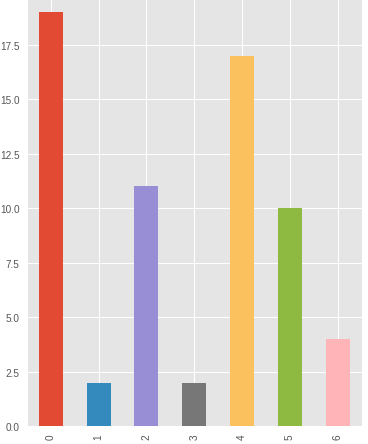
\includegraphics[width=58mm,scale=3]{sizez.png}
\caption{Sizes of each label}
\end{center}
\end{wrapfigure}

We have a visualization of the sizes for each label here corresponding to their label names. $x-$axis shows label-values that were coded and $y-$axis shows the respective sizes of each different label. With this bar graph we can comprehend that, \texttt{cold} and \texttt{fever} comprise a greater concentration in our data. Labels like \texttt{cold-fever} and \texttt{cold-soarthroat-fever} have the least number compared from the rest. Every column of the dataset is of numeric form except the \texttt{juice-names}. A machine learning model works smoothly only if the data is comprised of numbers, since we don't have numbers, we have \textit{integer-encode} that categorical columns. Integer encoding is a process of encoding text data into discrete numbers where in model does not face any impeding consequences during learning.
\paragraph{} Encoding was enforced with the help of a \texttt{Python} library named as \texttt{scikit-learn}, a Google Summer of Code project initiative which is open-source and serves substantial use-cases.
\end{document}
